% =============================================================================
%  SAMPLE COMPANION  —  a finished example built on templates/companion.tex
% =============================================================================
%  Works for ANY input: a topic, a list of topics, notes, a book chapter, a PDF
%  or a slide deck. Nothing here assumes slides exist.
%
%  THE LOOK (v3.1 "quiet" design): one ink colour + ONE accent colour. Calm,
%  editorial, lots of white space. No coloured fills, no rainbow of boxes.
%    * running header: series name (left) | topic title (right), small, grey
%    * title block: small accent label, large ink title, grey subtitle, hairline
%    * numbered sans section headings; the number in the accent colour
%    * SIX callouts, all the SAME shape: a thin accent rule on the left and a
%      small uppercase label. They differ by label, not by colour. Only the
%      worked example gets a faint grey wash, so it reads as "the work area".
%    * \housefig{path}{caption}: every figure the same width, caption below
%
%  BUILD:   python3 scripts/build_pdf.py output/<slug>/companion.tex
%
%  HOST AGENT: replace every {{PLACEHOLDER}}. The running header is driven by
%  two macros in the preamble (\SeriesName / \TopicTitle).
%  One specimen section is fully written so the template renders meaningfully.
%  Duplicate its structure per concept, then delete it.
% =============================================================================

\documentclass[a4paper,11pt]{article}

% ---- Encoding & fonts -------------------------------------------------------
\usepackage[T1]{fontenc}
\usepackage[utf8]{inputenc}
% Palatino text + matching math when available (ships with TeX Live's psnfss);
% falls back to Latin Modern on minimal installs. Helvetica for headings.
\IfFileExists{mathpazo.sty}{\usepackage[sc]{mathpazo}\linespread{1.06}}{\usepackage{lmodern}}
\IfFileExists{helvet.sty}{\usepackage[scaled=0.9]{helvet}}{}
\renewcommand{\ttdefault}{lmtt}     % Latin Modern mono: scalable, always present
\usepackage{microtype}              % protrusion/kerning -> fewer overfull boxes

% ---- Geometry ---------------------------------------------------------------
\usepackage[a4paper,top=26mm,bottom=26mm,left=27mm,right=27mm,
            headheight=14pt,headsep=12mm,footskip=12mm]{geometry}

% ---- Math -------------------------------------------------------------------
\usepackage{amsmath,amssymb}

% ---- Graphics, tables, colour ----------------------------------------------
\usepackage{graphicx}
\usepackage{booktabs}
\usepackage{array}
\usepackage[table,svgnames]{xcolor}
\usepackage{caption}
\usepackage{float}
\usepackage[section]{placeins}      % figures never drift into the next section
\usepackage{needspace}

% ---- Callout boxes ------------------------------------------------------------
\usepackage[most]{tcolorbox}
\tcbuselibrary{skins,breakable}

% ---- Tikz (ONLY for the specimen's inline sketch; real figs use \housefig) --
\usepackage{tikz}

% ---- Glyphs -----------------------------------------------------------------
\usepackage{pifont}

% ---- Lists & spacing --------------------------------------------------------
\usepackage{enumitem}
\setlist{leftmargin=1.5em,topsep=4pt,itemsep=3pt}

% ---- Dedicated "Step 1 / Step 2 ..." list for WORKED EXAMPLES ----------------
% Reserves label width so every "Step N" sits cleanly INSIDE the box, with the
% step text in a neat hanging column. ALWAYS use \begin{steps}...\end{steps}.
% NEVER write a raw \begin{enumerate}[label=\textbf{Step \arabic*.}] — it leaks.
\newlist{steps}{enumerate}{1}
\setlist[steps]{label={\sffamily\small\bfseries\color{accent}Step \arabic*},
  leftmargin=4.2em, labelwidth=3.6em, labelsep=0.6em, labelindent=0pt,
  align=left, topsep=6pt, itemsep=5pt}
\usepackage{parskip}                % blank-line paragraph spacing, no indent
\setlength{\parskip}{0.55em plus 0.1em}

% ---- Headers / footers ------------------------------------------------------
\usepackage{fancyhdr}

% ---- Section styling --------------------------------------------------------
\usepackage{titlesec}

% ---- Links (hidden) + URL line-breaking so long URLs never overflow ---------
\usepackage[hidelinks]{hyperref}
\usepackage{xurl}
\hypersetup{breaklinks=true}

% =============================================================================
%  COLOURS — ink, grey, ONE accent. That is the whole palette.
%  To re-theme a kit, change \definecolor{accent} only.
% =============================================================================
\definecolor{accent}{HTML}{1F4E79}      % deep blue: numbers, labels, rules
\definecolor{inktext}{HTML}{1F2328}     % body text
\definecolor{mutedtext}{HTML}{6B7280}   % header, captions, subtitles
\definecolor{hairline}{HTML}{D0D5DD}    % thin rules
\definecolor{wash}{HTML}{F5F6F8}        % the one fill (worked examples)
% Compatibility names (older kits and the specimen use these)
\colorlet{navy}{accent}      \colorlet{navyrule}{hairline}
\colorlet{intuFrame}{accent} \colorlet{everyFrame}{accent} \colorlet{workFrame}{accent}
\colorlet{watchFrame}{inktext} \colorlet{keyFrame}{accent} \colorlet{waitFrame}{accent}

\color{inktext}
\hypersetup{linkcolor=accent,urlcolor=accent,citecolor=accent}

% =============================================================================
%  RUNNING HEADER / FOOTER  (fancyhdr)  — every page
%  Left:  "Probability"      Right: "The Poisson Distribution"
%  SERIES_NAME is whatever frames the kit: a course name the user gave, a
%  series ("Study Companion"), or the subject area ("Linear Algebra").
% =============================================================================
\newcommand{\SeriesName}{Probability}          % e.g. "Study Companion"
\newcommand{\TopicTitle}{The Poisson Distribution}          % e.g. "Probability Distributions"

\pagestyle{fancy}
\fancyhf{}
\fancyhead[L]{\sffamily\scriptsize\color{mutedtext}\MakeUppercase{\SeriesName}}
\fancyhead[R]{\sffamily\scriptsize\color{mutedtext}\TopicTitle}
\fancyfoot[C]{\sffamily\footnotesize\color{mutedtext}\thepage}
\renewcommand{\headrulewidth}{0pt}
\renewcommand{\footrulewidth}{0pt}
\fancypagestyle{plain}{\fancyhf{}\fancyfoot[C]{\sffamily\footnotesize\color{mutedtext}\thepage}}

% =============================================================================
%  SECTION HEADINGS — sans, bold, ink; the number in the accent colour.
%  No heavy rules. Sections flow on (no forced page breaks, so no half-empty
%  pages); \needspace keeps a heading from stranding at a page bottom, and
%  placeins keeps each section's figures inside the section.
% =============================================================================
\titleformat{\section}
  {\sffamily\Large\bfseries\color{inktext}}
  {\color{accent}\thesection}{0.7em}{}
\titleformat{\subsection}
  {\sffamily\large\bfseries\color{inktext}}
  {\color{accent}\thesubsection}{0.6em}{}
\titlespacing*{\section}{0pt}{26pt}{6pt}
\titlespacing*{\subsection}{0pt}{14pt}{4pt}
\newcommand{\sectionbreak}{\needspace{14\baselineskip}}

% -----------------------------------------------------------------------------
%  \secsub{...} — the ONE-LINER under a section title.
%  Every section opens with the WHOLE idea in one or two plain sentences,
%  right under the heading, before any body prose. Write it as the claim the
%  section will prove, never as an agenda ("In this section we will...").
% -----------------------------------------------------------------------------
\newcommand{\secsub}[1]{%
  \noindent{\large\itshape\color{mutedtext}#1}\par
  \vspace{2pt}{\color{hairline}\rule{\linewidth}{0.4pt}}\par\medskip}

% -----------------------------------------------------------------------------
%  \flipanswer{...} — an upside-down answer for self-test questions.
% -----------------------------------------------------------------------------
\newcommand{\flipanswer}[1]{\par\noindent\hfill\rotatebox[origin=c]{180}{\parbox{0.9\linewidth}{\small\color{mutedtext}#1}}\par\medskip}

% =============================================================================
%  CALLOUTS — six environments, ONE shape.
%  A thin accent rule on the left, a small uppercase sans label on top, no fill.
%  They are told apart by the label. Only `worked` gets the faint grey wash.
%  Environment names are unchanged from earlier versions:
%     intuition · everyday · worked{caption} · watchout · waitwhat · keytake
% =============================================================================
\tcbset{
  quiet/.style 2 args={          % #1 = rule colour, #2 = background
    enhanced, breakable, sharp corners,
    colback=#2, colframe=#2, boxrule=0pt,
    borderline west={1.6pt}{0pt}{#1},
    left=12pt, right=10pt, top=7pt, bottom=7pt,
    before skip=12pt, after skip=12pt,
    fontupper=\normalsize, coltitle=#1,
    fonttitle=\sffamily\scriptsize\bfseries,
    attach title to upper={\par\smallskip},
  }
}
\newcommand{\calloutlabel}[1]{\MakeUppercase{#1}}

\newtcolorbox{intuition}{quiet={accent}{white},
  title={\calloutlabel{The intuition}}}
\newtcolorbox{everyday}{quiet={accent}{white},
  title={\calloutlabel{Everyday picture}}}
%  Usage: \begin{worked}{The caption}  ...steps...  \end{worked}
\newtcolorbox{worked}[1]{quiet={accent}{wash},
  title={\calloutlabel{Worked example}\ \textperiodcentered\ {\normalfont\itshape\small\color{inktext}#1}}}
\newtcolorbox{watchout}{quiet={inktext}{white},
  title={\calloutlabel{Watch out}}}
%  The honest surprise: one per concept AT MOST, only where a consequence is
%  genuinely startling. Never forced; an empty slot beats a fake surprise.
\newtcolorbox{waitwhat}{quiet={accent}{white},
  title={\calloutlabel{Wait --- really?}}}
\newtcolorbox{keytake}{quiet={accent}{white},
  borderline north={0.4pt}{0pt}{hairline},
  borderline south={0.4pt}{0pt}{hairline},
  title={\upshape\calloutlabel{Key takeaway}}, fontupper=\normalsize\itshape}

% =============================================================================
%  TITLE BLOCK  —  \titlebanner{LABEL}{TITLE}{SUBTITLE}{META LINE}
%  Quiet and typographic: accent label, big ink title, grey subtitle, hairline,
%  small grey meta line. No coloured slab.
% =============================================================================
\newcommand{\titlebanner}[4]{%
  \begingroup\raggedright
  \vspace*{4mm}
  {\sffamily\footnotesize\bfseries\color{accent}\MakeUppercase{#1}}\par
  \vspace{7pt}
  {\sffamily\bfseries\fontsize{30}{35}\selectfont\color{inktext}#2\par}
  \vspace{7pt}
  {\large\color{mutedtext}#3\par}
  \vspace{12pt}
  {\color{hairline}\rule{\linewidth}{0.5pt}}\par
  \vspace{3pt}
  {\sffamily\scriptsize\color{mutedtext}\MakeUppercase{#4}}\par
  \vspace{10pt}
  \endgroup
}

% =============================================================================
%  \housefig[width]{path}{caption}  —  one standard width (0.86\linewidth),
%  centred. Use the optional width (e.g. 0.55) only for small or tall figures
%  such as a 2x2 heatmap or a 3-D surface. Figures float to the nearest good
%  spot (top/bottom of the page) but never leave their section (placeins), so
%  pages stay full and aligned. Captions: small, grey, bold "Figure n".
% =============================================================================
\captionsetup[figure]{font={small,color=mutedtext},labelfont={bf,sf,color=inktext},
  labelsep=period,justification=raggedright,singlelinecheck=false,skip=6pt}
\setlength{\textfloatsep}{16pt plus 4pt minus 4pt}
\setlength{\intextsep}{14pt plus 4pt minus 4pt}
\renewcommand{\topfraction}{0.8}\renewcommand{\bottomfraction}{0.6}
\renewcommand{\textfraction}{0.15}\renewcommand{\floatpagefraction}{0.75}
\newcommand{\housefig}[3][0.86]{%
  \begin{figure}[!htbp]
    \centering
    \includegraphics[width=#1\linewidth]{#2}%
    \caption{#3}
  \end{figure}%
}

% Tables: small, sans headers, a little more row air.
\renewcommand{\arraystretch}{1.18}

% A small inline-vocabulary helper: first use of a term.
\newcommand{\vocab}[1]{\textbf{#1}}

% =============================================================================
%  OVERFLOW-SAFETY CHEAT-SHEET (read before filling)
% =============================================================================
%  * WIDE MATH: never one long line. Wrap with align / split / multline.
%  * WIDE TABLE: \resizebox{\linewidth}{!}{\begin{tabular}...\end{tabular}}
%        (or booktabs columns sized with p{..} that sum under \linewidth).
%  * LONG URL: \url{...} (xurl lets it break anywhere).
%  * FIGURES: always \housefig — never a raw oversized box.
%  * WORKED-EXAMPLE STEPS: ALWAYS use \begin{steps}...\end{steps}.
%  * CONTENT INSIDE A BOX must fit the box: a wide table or long equation in a
%        callout still needs \resizebox / align.
% =============================================================================

% Older sample environment names, mapped onto the six template callouts.
\newenvironment{intuitionbox}{\begin{intuition}}{\end{intuition}}
\newenvironment{everydaybox}{\begin{everyday}}{\end{everyday}}
\newenvironment{workedbox}[1]{\begin{worked}{#1}}{\end{worked}}
\newenvironment{watchoutbox}{\begin{watchout}}{\end{watchout}}
\newenvironment{keytakebox}{\begin{keytake}}{\end{keytake}}
\colorlet{cWork}{accent}

\begin{document}

\thispagestyle{fancy}
\titlebanner
  {\SeriesName}
  {Poisson: counting rare events}
  {The distribution of ``how many happened'' when each one is rare.}
  {Built from: the topic ``Poisson distribution'' \textperiodcentered\ Every example worked out in full}

\noindent\textbf{How to use this companion.}
This companion explains the idea from scratch, in plain English. Small labels
mark the boxes. \textsf{\small\textbf{THE INTUITION}} explains an idea in plain
words. \textsf{\small\textbf{EVERYDAY PICTURE}} ties it to real life.
\textsf{\small\textbf{WORKED EXAMPLE}}, on a grey background, solves a problem
with real numbers, every step shown. \textsf{\small\textbf{WATCH OUT}} flags a
common mistake. \textsf{\small\textbf{KEY TAKEAWAY}} is the one line to remember.

% ============================================================================
\section{The big idea: counting rare events in a fixed window}
% ============================================================================

A \emph{Poisson distribution} answers one question: in a fixed stretch of time
or space, how many times does a rare event happen? Think of calls to a help
desk in one hour, or typos on one page. We do not ask \emph{when} each one
happens. We only count \emph{how many}.

The whole distribution rides on a single number, $\lambda$ (the Greek letter
"lambda"). Here $\lambda$ is the \textbf{average count} you expect in that
window. If a help desk gets $3$ calls per hour on average, then $\lambda = 3$
for a one-hour window. That is all you need.

\begin{intuitionbox}
Picture a long, quiet afternoon at a shop. Customers trickle in at random.
There is no schedule and no pattern. You cannot say "the next one comes at
2:40". But you \emph{can} say "about $4$ per hour, on average". The Poisson
distribution turns that one average, $\lambda$, into the full odds: the chance
of seeing exactly $0$, exactly $1$, exactly $2$ customers, and so on. One
number in; a whole table of probabilities out.
\end{intuitionbox}

\begin{everydaybox}
Think of rain hitting a single floor tile during a light drizzle. Drops land at
random spots and random moments. Stand over one tile for ten seconds and count
the hits. Some ten-second spells catch $0$ drops, some catch $1$, a few catch
$3$ or $4$. The \emph{average} hits per ten seconds is steady; the
\emph{exact} count jumps around. That jumpy count is exactly a Poisson count.
\end{everydaybox}

Now the formula. The probability of seeing exactly $k$ events is
%
\begin{equation}
  P(X = k) \;=\; \frac{\lambda^{k}\, e^{-\lambda}}{k!},
  \qquad k = 0, 1, 2, \dots
  \label{eq:poisson}
\end{equation}
%
Let us name every symbol, slowly:
\begin{itemize}
  \item $X$ is the random count — the number we do not yet know.
  \item $k$ is one specific count we ask about, like "exactly $2$".
  \item $\lambda$ is the average count in the window (here, a positive number).
  \item $e \approx 2.71828$ is Euler's number, a fixed constant.
  \item $k! = k \times (k{-}1) \times \cdots \times 2 \times 1$ is "$k$
        factorial", and we set $0! = 1$ by convention.
\end{itemize}

\noindent Two facts make this easy to use. For a Poisson count, the
\textbf{mean} (average) and the \textbf{variance} (spread) are \emph{both} equal
to $\lambda$:
%
\begin{equation}
  \mathbb{E}[X] = \lambda,
  \qquad
  \operatorname{Var}(X) = \lambda .
  \label{eq:meanvar}
\end{equation}
%
So one number sets both the centre and the width of the distribution.

% ----------------------------- WORKED EXAMPLE -------------------------------
\begin{workedbox}{help-desk calls in one hour}
A help desk receives $\lambda = 3$ calls per hour on average. What is the
probability of getting \emph{exactly} $2$ calls in the next hour? Then, what is
the probability of getting \emph{at least} $1$ call?
\begin{steps}
  \item \textbf{Write down what we know.} The average is $\lambda = 3$. We want
        $P(X = 2)$, so the specific count is $k = 2$.
  \item \textbf{Plug into the formula \eqref{eq:poisson}.} Substituting
        $\lambda = 3$ and $k = 2$:
        \[
          P(X = 2) = \frac{3^{2}\, e^{-3}}{2!}.
        \]
  \item \textbf{Work out each piece.} The top has $3^{2} = 9$. The factorial is
        $2! = 2 \times 1 = 2$. The constant is $e^{-3} \approx 0.049787$.
  \item \textbf{Combine the numbers.}
        \[
          P(X = 2)
          = \frac{9 \times 0.049787}{2}
          = \frac{0.448083}{2}
          = 0.224042.
        \]
        So there is about a $\mathbf{22.4\%}$ chance of exactly two calls.
  \item \textbf{Now the "at least one" part.} "At least $1$" is the opposite of
        "exactly $0$". So compute $P(X = 0)$ first and subtract from $1$:
        \[
          P(X = 0) = \frac{3^{0}\, e^{-3}}{0!}
                   = \frac{1 \times 0.049787}{1}
                   = 0.049787.
        \]
  \item \textbf{Subtract.}
        \[
          P(X \ge 1) = 1 - P(X = 0)
                     = 1 - 0.049787
                     = 0.950213.
        \]
        So there is about a $\mathbf{95.0\%}$ chance of \emph{at least} one call.
\end{steps}
Notice the "at least" trick: instead of adding up $P(1) + P(2) + P(3) + \cdots$
forever, we used one easy subtraction. That shortcut works whenever "at least
one" is the goal.
\end{workedbox}

\begin{watchoutbox}
$\lambda$ must match your \emph{window}. The $3$ calls were \emph{per hour}. If
you ask about a $20$-minute window instead, scale $\lambda$ to that window
first: $20$ minutes is $\tfrac{1}{3}$ of an hour, so use $\lambda = 3 \times
\tfrac{1}{3} = 1$. Plugging the hourly $\lambda = 3$ into a $20$-minute question
silently inflates every probability. Always rescale $\lambda$ to the window you
are actually asking about.
\end{watchoutbox}

% ----------------------------- TIKZ MINI-FIGURE -----------------------------
\begin{center}
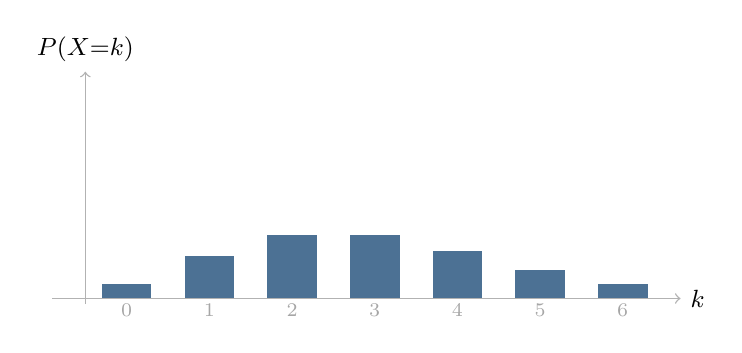
\begin{tikzpicture}[x=1.05cm,y=3.6cm]
  % axes
  \draw[->,gray!60,line width=0.5pt] (-0.4,0) -- (7.2,0) node[right,black,font=\small]{$k$};
  \draw[->,gray!60,line width=0.5pt] (0,-0.02) -- (0,0.80) node[above,black,font=\small]{$P(X{=}k)$};
  % Poisson(3) bars, heights = probabilities, drawn to scale (max ~0.224 at k=2,3)
  \foreach \k/\p in {0/0.0498,1/0.1494,2/0.2240,3/0.2240,4/0.1680,5/0.1008,6/0.0504}{
    \fill[accent!80] (\k+0.20,0) rectangle (\k+0.80,\p);
    \node[font=\scriptsize,gray!70] at (\k+0.5,-0.04) {\k};
  }
\end{tikzpicture}
\end{center}

\noindent The bars are tallest around $k = 2$ and $k = 3$, right next to the
average $\lambda = 3$, then fade out for large $k$. A rare-event count clusters
near its mean and rarely strays far.

\begin{keytakebox}
One number, $\lambda$, is the whole story. It is the average count, and (by
\eqref{eq:meanvar}) also the variance. Feed it into
$P(X{=}k)=\lambda^{k}e^{-\lambda}/k!$ to get the chance of any exact count.
Always match $\lambda$ to your window, and use the "$1 - P(0)$" trick for "at
least one".
\end{keytakebox}

% ----------------------------- WHERE IT'S USED ------------------------------
\noindent\textbf{Where it's used.}
Poisson counts are the backbone of \emph{Poisson regression}, used to model
count targets — clicks on an ad, support tickets per day, goals in a match.
There the model predicts $\lambda = e^{\,\boldsymbol{\beta}^{\!\top}\mathbf{x}}$
from features $\mathbf{x}$, so $\lambda$ stays positive and the loss is the
Poisson negative log-likelihood. The same distribution underlies the Poisson
layer in deep count models and the noise model for photon-limited images.

\end{document}
